% !TEX root = ./main.tex
\graphicspath{{figures_flatplate/}}% Set graphics path location

\subsection{Subsonic laminar flat-plate}

Computations of the flow over a subsonic flat-plate have been performed and validated against the Blasius' solution for laminar boundary layer. The flow conditions are Mach number $0.5$, angle of attack $0.0\deg$ and Reynolds number based on the plate length of $1\cdot10^6$. The governing equations are the 2D Navier-Stokes equations with constant ratio of specific heats of $1.4$, Prandtl number of $0.72$ and constant dynamic viscosity of $1.827\cdot 10^{-5} Pa \cdot s$.

\begin{center} 
    \begin{tabular}{l*{5}{c}r}
    Height first cell \& \# of cells inside the boundary layer & Poly order 3 & Poly order 4 & Poly order 5 & Poly order 6 \\ \hline
    Mesh a0 (140 = 14x10). 0.00075 / 2 cells & $\times$ & $\times$ & $\times$ & \Checkmark \\ \hline
    Mesh a1 (560 = 28x20). 0.000375 / 4 cells &  $\times$ & $\times$ & \Checkmark & \Checkmark \\ \hline
    Mesh a2 (2240 = 56x40). 0.0001875  / 8 cells & $\times$ & \Checkmark & \Checkmark & \Checkmark \\ \hline
    Mesh a3 (8960 = 112x80). 0.0000935  / 16 cells & \Checkmark & \Checkmark & \Checkmark & \Checkmark \\
    \hline
    \end{tabular} 
      \captionof{table}{HiFiLES convergence using different grids and polynomial order} \label{table:convergence} 
\end{center}

The objective of this study is to determine the minimum number of elements and the order of polynomial required to converge the flat-plate simulation using HiFILES. In particular, 4 different numerical grids have been used in this study (2, 4, 8, 16 elements inside the boundary layer). The results are summarized in Table \ref{table:convergence}, the simulations require a minimum number of elements in the boundary layer to obtain a satisfactory converge, otherwise, there will be noticeable jumps across the elements.

\begin{figure}
\begin{center}
\begin{minipage}[t]{0.48\columnwidth}
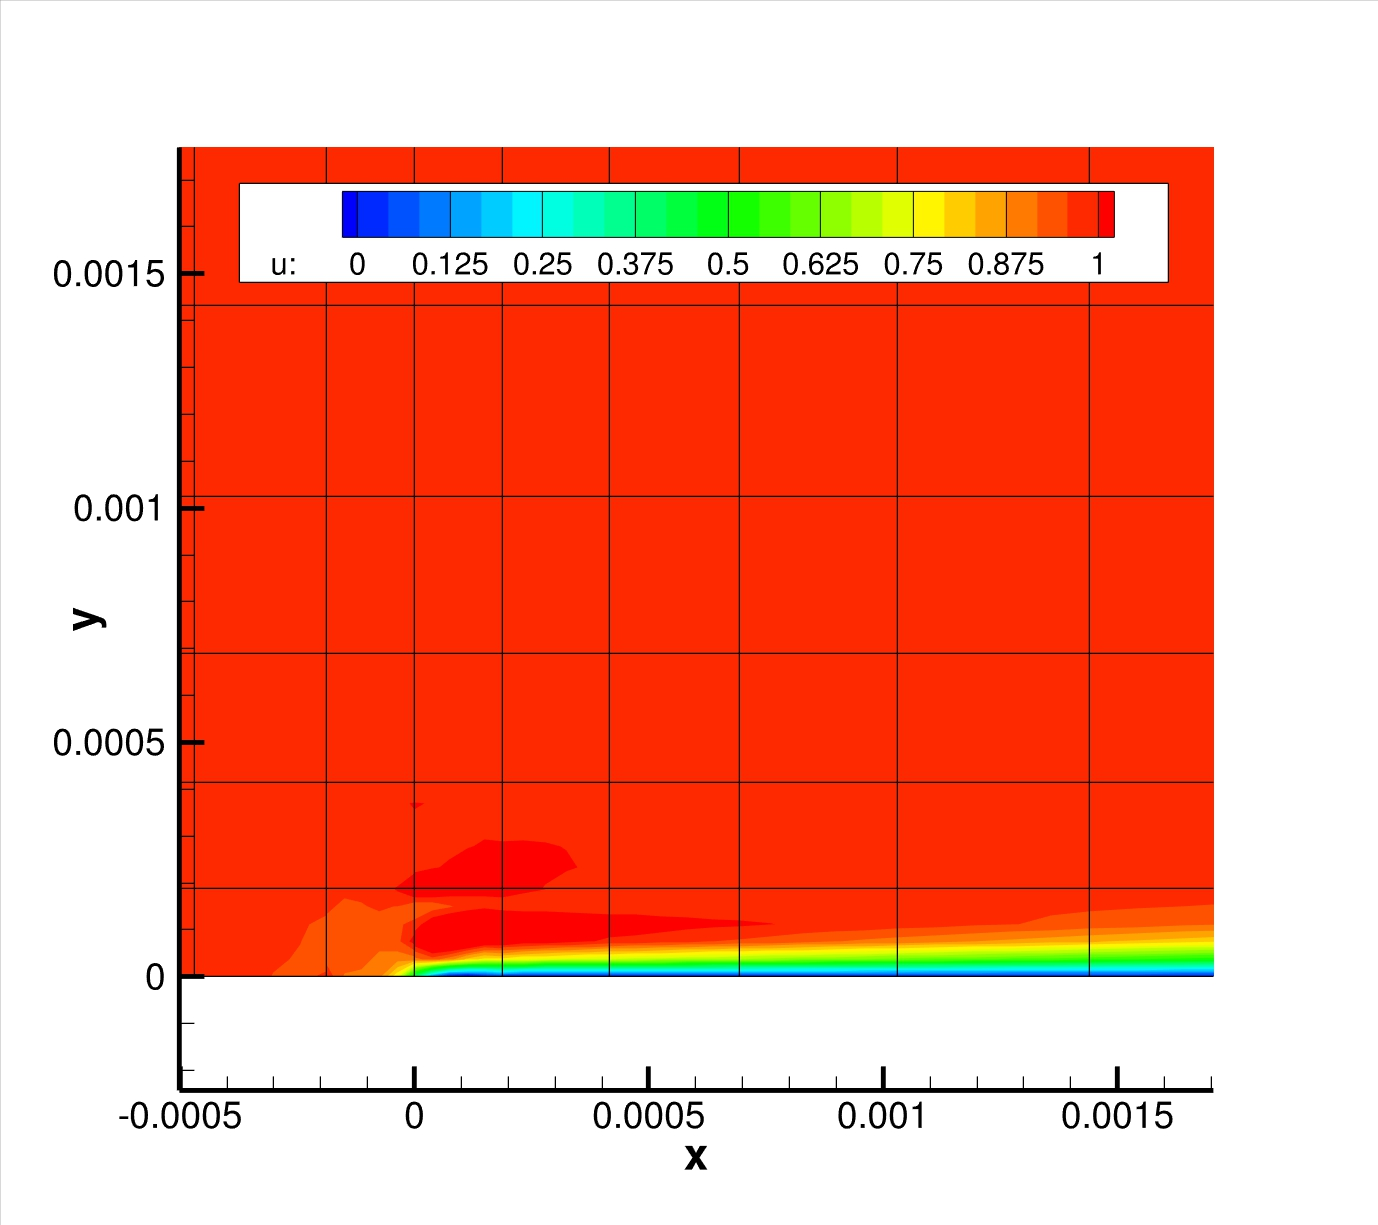
\includegraphics[width = \textwidth,clip=]{LeadingEdge.jpg}
\caption{Detail of the flat-plate leading edge (x=0.0, mesh a2).}
\label{fig:LeagingEdge}
\end{minipage}
\hfill
\begin{minipage}[t]{0.48\columnwidth}
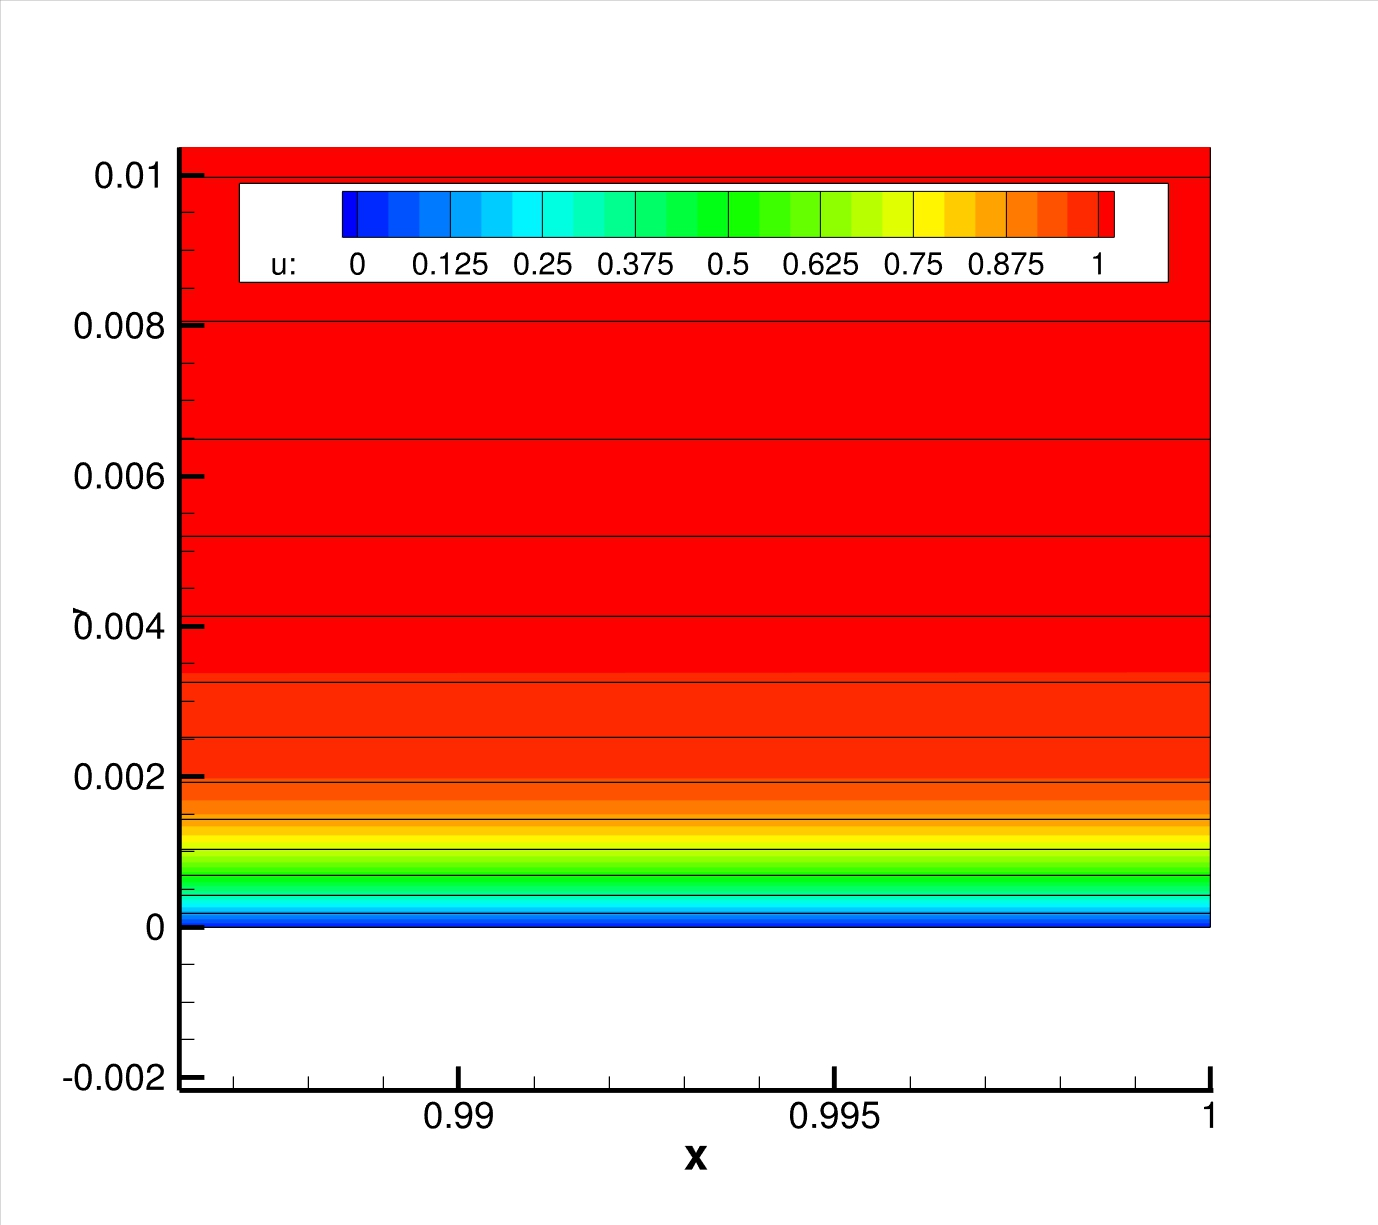
\includegraphics[width = \textwidth,clip=] {EndPlate.jpg}
\caption{Flow solution at the end of the flat-plate (x=1.0, mesh a2).}
\label{fig:TrailingEdge}
\end{minipage}
\end{center}
\end{figure}

The results has been compared with the Blasius' solution for laminar boundary layer with satisfactory results, and some details of the solutions are presented in Fig. \ref{fig:LeagingEdge} (leading edge), and Fig. \ref{fig:TrailingEdge} (end of the flat-plate). It is important to note that in this particular case (mesh a2) the flap-plate is captured using 8 elements, while in a second order solver it would be necessary of the order of ~30 elements inside the boundary layer.

\begin{figure}
\begin{center}
\begin{minipage}[t]{0.48\columnwidth}
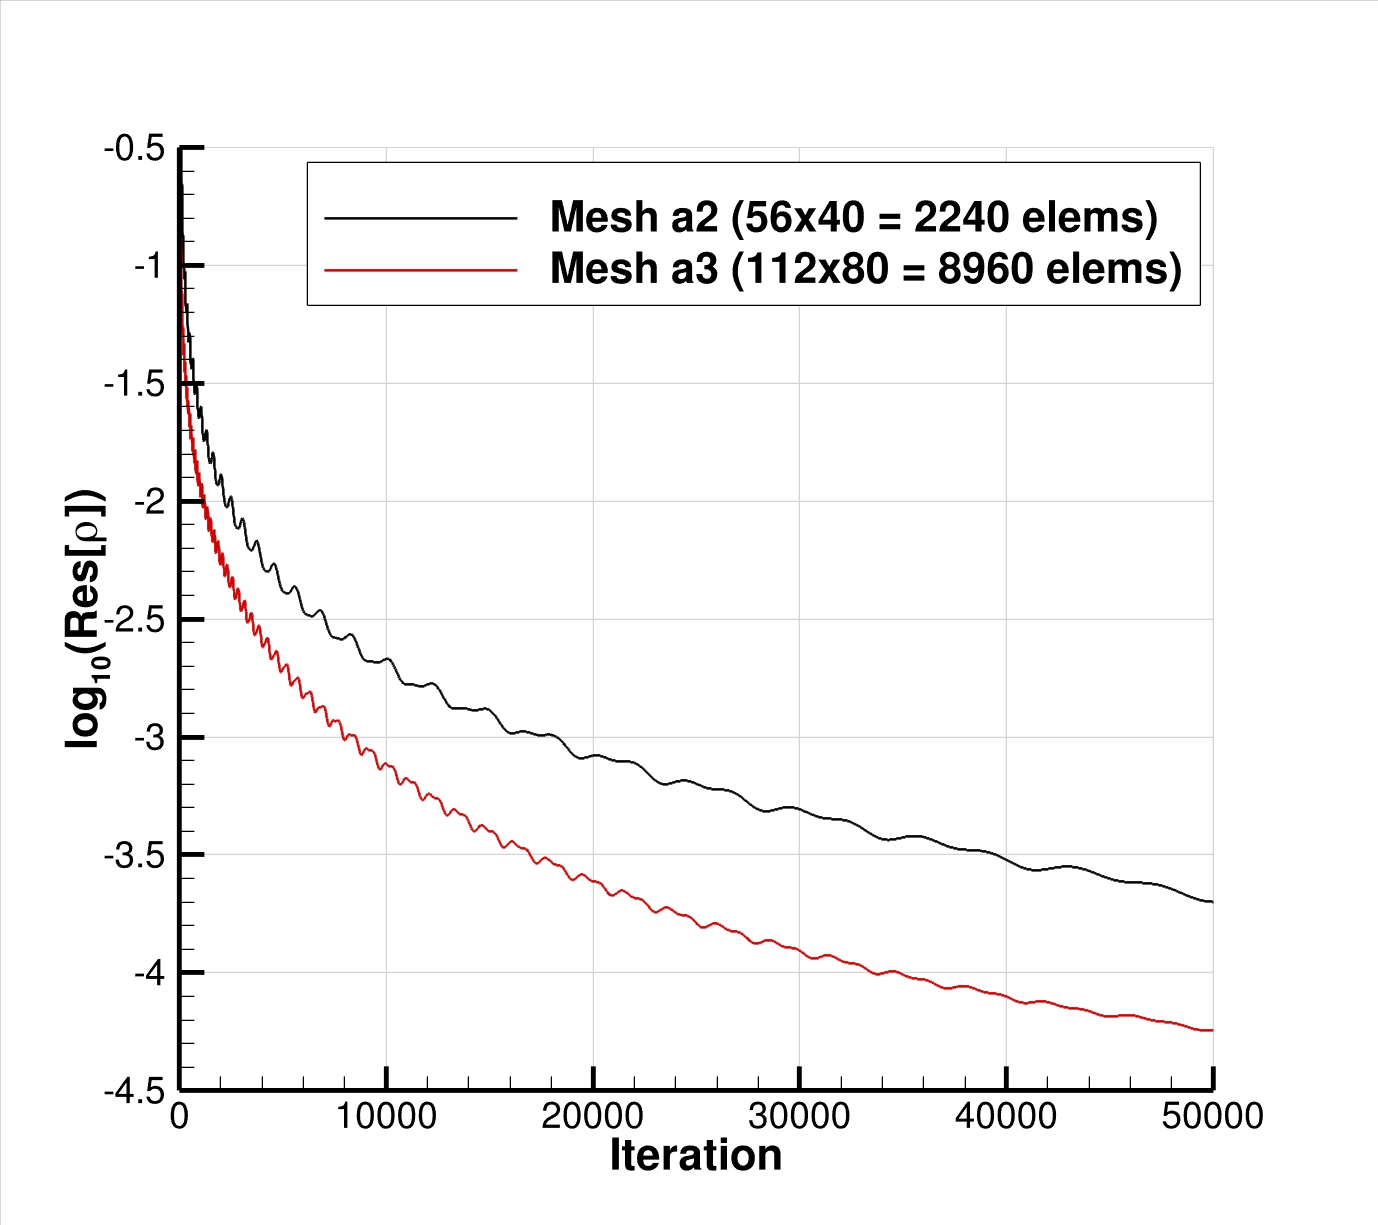
\includegraphics[width = \textwidth,clip=]{CompMesh.jpg}
\caption{Convergence comparison (3$^rd$ order, finest grids).}
\label{fig:ComparisonOrder}
\end{minipage}
\hfill
\begin{minipage}[t]{0.48\columnwidth}
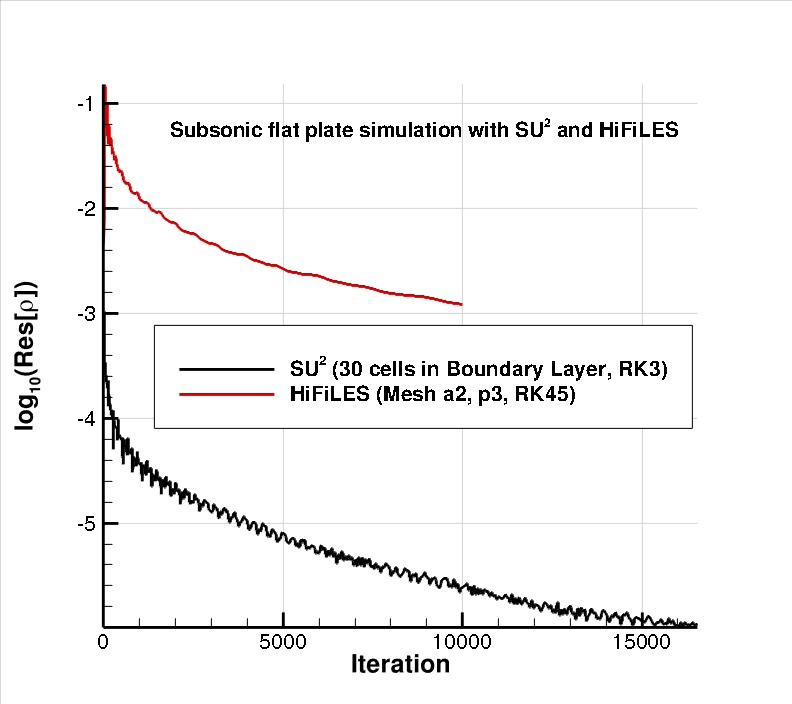
\includegraphics[width = \textwidth,clip=] {CompSu2.jpg}
\caption{Comparison of HiFiLES with SU$^2$ using a similar time integration scheme.}
\label{fig:Comparison_SecondOrder}
\end{minipage}
\end{center}
\end{figure}

To finalize, it is critical to note that the absence of a local time stepping technique in HiFiLES increases the required number of iterations to obtain a converged solution. However, we have noticed an improvement of the rate of converge as we refine the grid (see Fig. \ref{fig:ComparisonOrder}). Finally, the obtained convergence rate is comparable to a second order numerical code (e.g. SU$^2$\cite{palacios13,palacios14}) running using a similar numerical time integration (see Fig.\ref{fig:Comparison_SecondOrder}).
